\section{Figures} % (fold)
\label{sec:list_of_figures}


\begin{figure}[h!]
	\begin{tabular}{|p{\textwidth}|}
		\hline
		\begin{verbatim}
			var file = new File(filename);
			var metadata_group = file.GetGroup("metadata");
			var song_data = metadata_group.GetCompoundDataset("songs");
			string artist_name = song_data[0].GetString("artist_name");
		\end{verbatim} \\
		\hline
	\end{tabular}
	\caption{Example of syntax built to read HDF5 files (found in the \emph{HDF5Reader} library).}
    \label{fig:hdf5-syntax}
\end{figure}

\vspace{2.3cm}
\begin{figure}[h!]
	\centering
	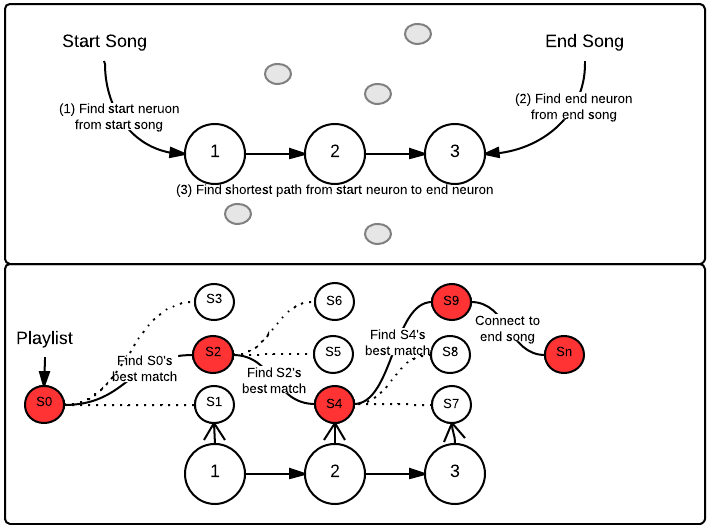
\includegraphics[width=\textwidth]{figures/playlist-generation}
	\caption{Illustration of the playlist algorithm.}
    \label{fig:playlist-gen}
\end{figure}

\newpage

\begin{figure}[h!]
    \centering
    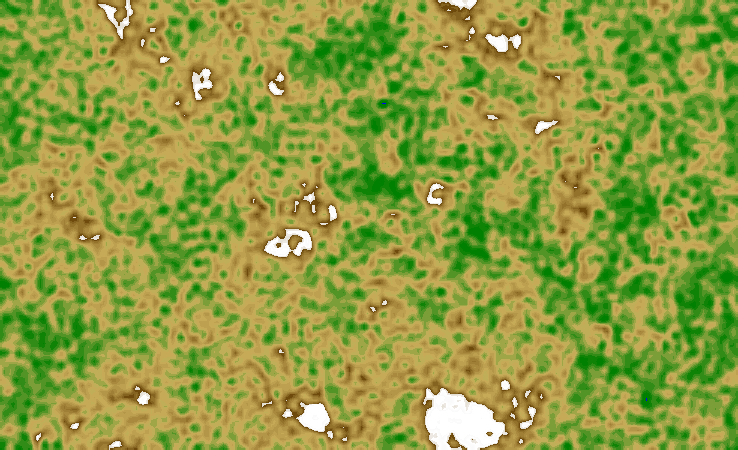
\includegraphics[angle=90, width=0.9\textwidth]{figures/map.jpg}
    \caption{U-matrix visualisation of the SOM, after training with 10.000 songs}
    \label{fig:map}
\end{figure}

%\newgeometry{left=2cm}

\begin{figure}[h!]
    \centering
    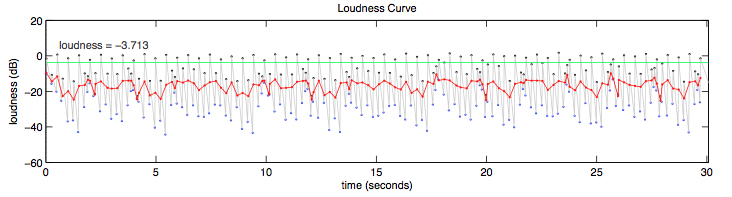
\includegraphics[width=\textwidth]{figures/loudness.jpg}
    \caption{Graphical representation of the loudness attributes of the segments from 39 seconds of "Around The World" by Daft Punk.}
    \label{fig:loudness}
\end{figure}

\vspace{2cm}

\begin{figure}[h!]
    \centering
    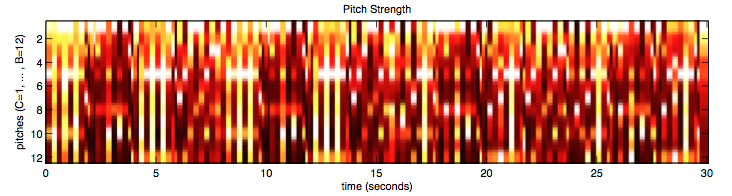
\includegraphics[width=\textwidth]{figures/pitch.jpg}
    \caption{Graphical representation of the ptich vector attributes of the segments from 39 seconds of "Around The World" by Daft Punk.}
    \label{fig:pitch}
\end{figure}

\vspace{1cm}

\begin{figure}[h!]
    \centering
    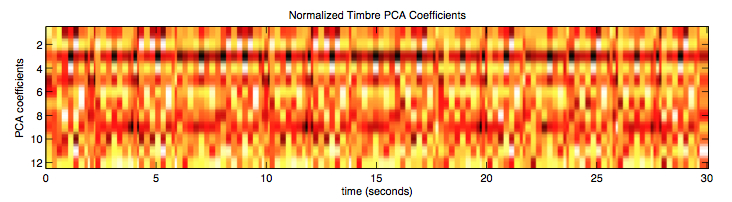
\includegraphics[width=\textwidth]{figures/timbre.jpg}
    \caption{Graphical representation of the timbre vector attributes of the segments from 39 seconds of "Around The World" by Daft Punk.}
    \label{fig:timbre}
\end{figure}
\newpage
%\restoregeometry

\begin{figure}[h!]
    \centering
    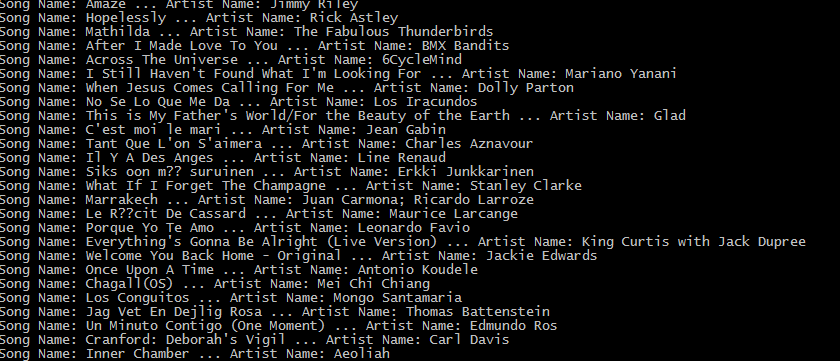
\includegraphics[width=\textwidth]{figures/ESOMSongs.PNG}
    \caption{Playlist description with ESOM path generation}
    \label{fig:esomres}
\end{figure}

\begin{figure}[h!]
    \centering
    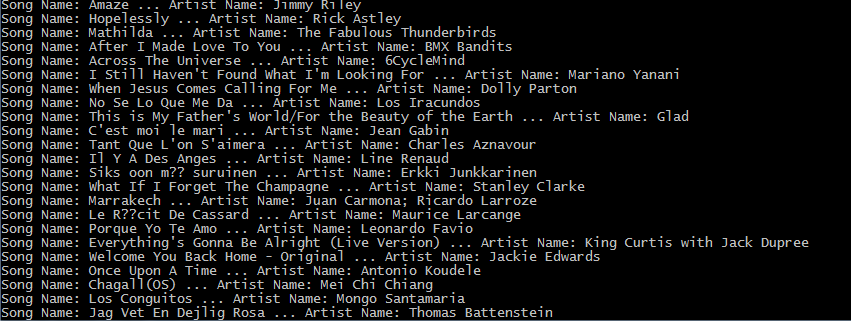
\includegraphics[width=\textwidth]{figures/UMatSongs.PNG}
    \caption{Playlist description with UMat path generation}
    \label{fig:umatres}
\end{figure}
% section list_of_figures (end)